% sage_latex_guidelines.tex V1.20, 14 January 2017

\documentclass[Review,sagev,times]{sagej}
%\documentclass[Afour,sagev,times]{sagej}

\usepackage{moreverb,url}

\usepackage[colorlinks,bookmarksopen,bookmarksnumbered,citecolor=red,urlcolor=red]{hyperref}
\usepackage{caption}
\usepackage{pdfpages}
\usepackage[tbtags]{amsmath}

\PassOptionsToPackage{tbtags}{amsmath}

\newcommand\BibTeX{{\rmfamily B\kern-.05em \textsc{i\kern-.025em b}\kern-.08em
T\kern-.1667em\lower.7ex\hbox{E}\kern-.125emX}}

\DeclareMathOperator{\argmax}{arg\,max}

\def\volumeyear{2018}

\begin{document}

\runninghead{Tomer et al.}

\title{Personalized Decision Making for Biopsies in Prostate Cancer Active Surveillance Programs}

\author{Anirudh Tomer\affilnum{1}, Dimitris~Rizopoulos\affilnum{1}, Daan~Nieboer\affilnum{2}, Frank-Jan~Drost\affilnum{3}, Monique~J.~Roobol\affilnum{3}, and Ewout~W.~Steyerberg\affilnum{2,4}}

\affiliation{\affilnum{1}Department of Biostatistics, Erasmus University Medical Center, the Netherlands\\
\affilnum{2}Department of Public Health, Erasmus University Medical Center, the Netherlands\\
\affilnum{3}Department of Urology, Erasmus University Medical Center, the Netherlands\\
\affilnum{4}Department of Biomedical Data Sciences, Leiden University Medical Center, the Netherlands}

\corrauth{Anirudh Tomer, 
Erasmus MC,
t.a.v. Anirudh Tomer / kamer flex Na-2823,
PO Box 2040,
3000 CA Rotterdam,
the Netherlands.}

\email{a.tomer@erasmusmc.nl}

% !TEX root =  ../main_manuscript.tex 
\begin{abstract}
\texttt{Background}: Prostate cancer active surveillance (AS) patients undergo repeat biopsies. Active treatment is advised when biopsy Gleason grade group~$\geq$~2 (\textit{upgrading}). Many patients never experience upgrading, yet undergo biopsies frequently. Personalized biopsy decisions based on upgrading-risk may reduce patient burden.\\

\texttt{Objective}: Develop a risk prediction model and web-application to assist patients/doctors in personalized biopsy decisions.\\

\texttt{Design, Setting, and Participants}: Model development: world's largest AS study PRIAS, 7813 patients, 1134 experienced upgrading; External validation: largest five cohorts of Movember Foundation's GAP3 database (${>20,000}$ patients, 27 centers worldwide); Data: repeat prostate-specific antigen (PSA) and biopsy Gleason grade.\\

\texttt{Outcome Measurements, and Statistical Analysis}: A Bayesian joint model fitted to the PRIAS dataset. This model was validated in GAP3 cohorts using risk prediction error, calibration, area under ROC (AUC). Model and personalized biopsy schedules based on predicted risks were implemented in a web-application.\\

\texttt{Results and Limitations}: Cause-specific cumulative upgrading-risk at year five of follow-up: 35\% in PRIAS, at most 50\% in GAP3 cohorts. PRIAS based model: PSA velocity was a stronger predictor of upgrading (Hazard~Ratio:~2.47, 95\%CI:~1.93--2.99) than PSA value (Hazard~Ratio:~0.99, 95\%CI:~0.89--1.11). Validation: Moderate AUC (0.55--0.75) in PRIAS and GAP3 cohorts. Moderate prediction error (0.1--0.3) in GAP3 cohorts where impact of PSA value and velocity on upgrading-risk was similar to PRIAS, but large (0.3--0.45) otherwise. Recalibration advised for external cohorts.\\

\texttt{Conclusions}: We successfully developed and validated a model for predicting upgrading-risk, and providing risk-based personalized biopsy decisions, in prostate cancer AS. The model made available via a web-application enables shared decision making of biopsy schedules by comparing fixed and personalized schedules on total biopsies and expected time delay in detecting upgrading.\\

\texttt{Patient Summary}: Personalized prostate biopsies are a novel alternative to fixed one-size-fits-all schedules. The underlying statistical models are made available through a user-friendly web-application and may help to reduce unnecessary prostate biopsies while maintaining cancer control.
\end{abstract}

\keywords{Active~surveillance, biopsy, joint~models, personalized~medical~decisions, prostate~cancer}

\maketitle

\footnote{Financial support for this study was provided entirely by a) VIDI grant nr. 016.146.301 from Nederlandse Organisatie voor Wetenschappelijk Onderzoek, which is the national research council of the Netherlands, and b) Erasmus University Medical Center funding. The funding agreement ensured the authors’ independence in designing the study, interpreting the data, writing, and publishing the report.\\Word count: 4085}
\thefootnote

% !TEX root =  ../main_manuscript.tex 
\section{Introduction}
Patients with low- and very low-risk screening-detected localized prostate cancer are usually advised active surveillance (AS) instead of immediate radical treatment~\citep{briganti2018active}. In AS, cancer progression is routinely monitored via prostate-specific antigen (PSA), digital rectal examination, and repeat biopsies. Among these, the strongest indicator of cancer-related outcomes is the biopsy Gleason grade~\citep{epsteinGG2014}. When the Gleason grade increases from grade~1 (Gleason 3+3) to 2 (Gleason 3+4) or higher, called \textit{reclassification}, patients are commonly advised curative treatment~\citep{bul2013active}.

\begin{figure}
\centerline{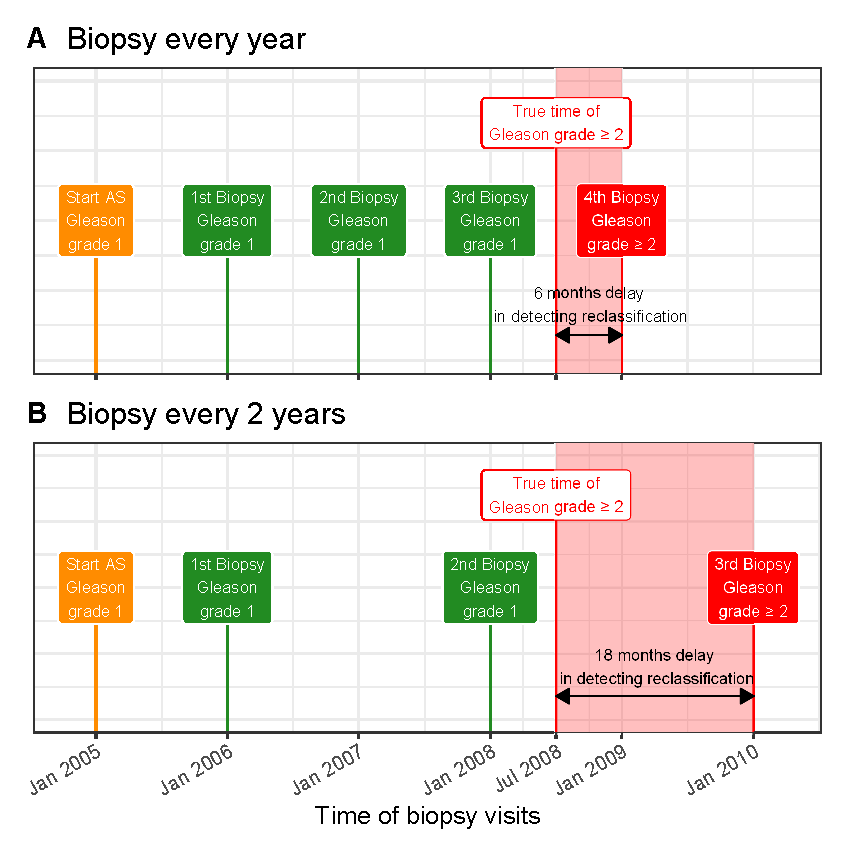
\includegraphics[width=\columnwidth]{images/delay_explanation.eps}}
\caption{\textbf{Trade-off between the number of biopsies and time delay in detecting reclassification (Increase in Gleason grade from 1 to 2 or higher):} The true time of reclassification for the patient in this figure is July 2008. When biopsies are scheduled annually (\textbf{Panel~A}), reclassification is detected in January 2009 with a time delay of six months, and a total of four biopsies are scheduled. When biopsies are scheduled biennially (\textbf{Panel~B}) reclassification is detected in January 2010 with a time delay of 18 months, and a total of three biopsies are scheduled. Since biopsies are conducted periodically, the time of reclassification is observed as an interval. For example, between Jan~2008--Jan~2009 in \textbf{Panel~A} and between Jan~2008--Jan~2010 in \textbf{Panel~B}.}
\label{fig:delay_explanation}
\end{figure}

Biopsies are conducted periodically. Consequently, reclassification is always detected with a time delay (Figure~\ref{fig:delay_explanation}). For detecting reclassification timely, many AS programs schedule fixed and frequent biopsies (e.g.,~annually) for all patients~\citep{nieboer2018active,loeb2014heterogeneity}. However, this also leads to many unnecessary biopsies in slow/non-progressing patients. Biopsies are invasive, painful and prone to medical complications. Thus, biopsy burden and patient non-compliance to frequent biopsies~\citep{bokhorst2015compliance} has raised concerns regarding the optimal biopsy schedule~\citep{inoue2018comparative, bratt2013study}. To this end, infrequent schedules such as biennial biopsies have been proposed as an alternative~\citep{inoue2018comparative,de2017estimating}. Although, biennial biopsies may still lead to five unnecessary biopsies over ten years (current study period of large AS programs) for slow/non-progressing patients. A promising alternative to fixed and frequent biopsies is personalized biopsy schedules based on the patient-specific risk of reclassification (Figure~\ref{fig:riskBasedExample}).

\begin{figure}
\centerline{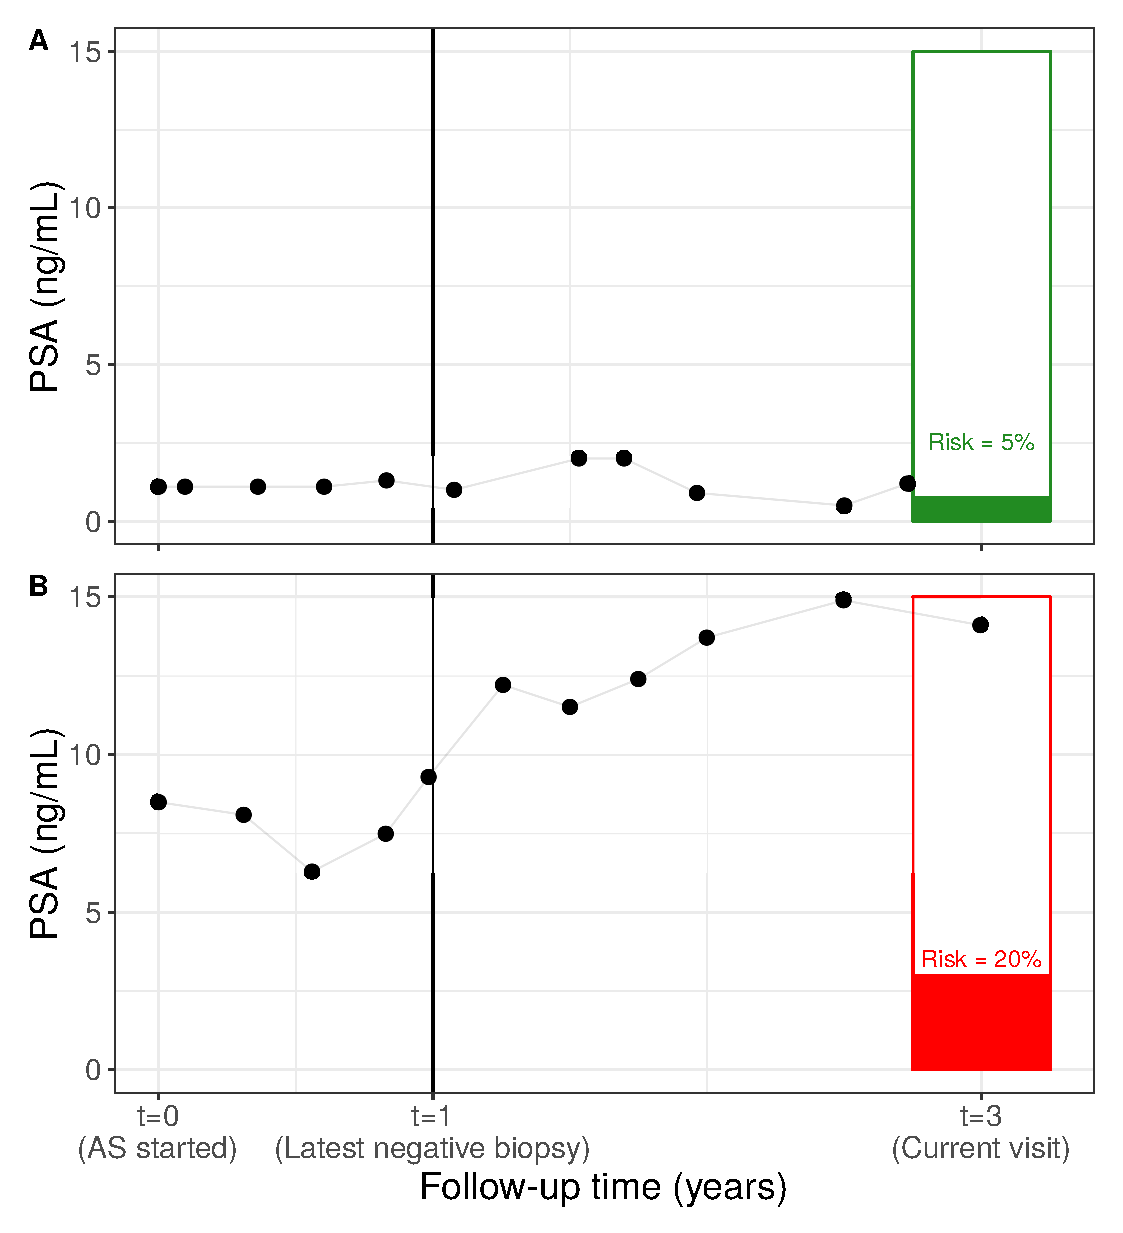
\includegraphics[width=\columnwidth]{images/riskBasedExample.eps}}
\caption{\textbf{Motivation for personalized risk-based decisions of biopsy}: Patient~A (\textbf{Panel~A}) and B (\textbf{Panel~B}) had their latest biopsy at year one of follow-up (green vertical line). Patient~A's prostate-specific antigen (PSA) profile remained stable until his current visit at year three, whereas patient~B's profile has shown a rise. Consequently, patient~B's estimated cumulative risk of reclassification at the current visit (year three) is higher than that of patient~A. This makes patient~B a more suitable candidate for biopsy than Patient~A. Risk estimates in this figure are only illustrative.}
\label{fig:riskBasedExample}
\end{figure}

The first challenge in developing personalized biopsy schedules is consolidating accumulated patient data (e.g., PSA, previous biopsy results) into risk estimates for reclassification. Existing calculators for risk of reclassification~\citep{partin1993use,makarov2007updated} use only the latest PSA measurement of a patient. In contrast, we intend to utilize all repeated measurements of PSA, previous biopsy results, and baseline characteristics of a patient. To this end, a suitable model is the joint model for time-to-event and longitudinal data~\citep{tomer2019, coley2017prediction,rizopoulos2012joint}. A joint model predicts risk of reclassification in a personalized manner. A subsequent challenge however, is translating risks into clinical decisions. For example, a 10\% risk of reclassification can be perceived high/low depending upon the patient age. Patients may also weigh risks of reclassification with the potential \textit{consequences} of another biopsy. Two relevant \textit{consequences} of biopsies (Figure~\ref{fig:delay_explanation}) are the timing and total number of biopsies (burden), and the time delay in detecting reclassification (smaller is beneficial). The relative importance of these \textit{consequences} can vary between the patients, and also over the follow-up period for the same patient.

The goal of this work was to assist patients and doctors in making better decisions of biopsies than fixed and frequent biopsies. For this purpose, we developed a web-application that gives patients their current and future risk of reclassification. It also suggests them risk-based personalized schedules of biopsies. For each biopsy schedule, be it fixed or personalized, the web-application provides expected \textit{consequences} of following it. Thus, patients can compare schedules before making a decision. The web-application uses a prediction joint model fitted to the world's largest AS dataset, PRIAS~\citep{bul2013active}. We externally validated this model in five largest AS cohorts of the GAP3 database \citep{gap3_2018}. Thus, the web-application can be used by a large number of patients worldwide.

\section{Methods}
\label{sec:methods}
% !TEX root =  ../main_manuscript.tex

\subsection{Study Population}
\label{subsec:study_population}
To develop our methodology we use the data of prostate cancer patients from the world's largest AS study called PRIAS \cite{bokhorst2016decade} (see Table \ref{table:prias_summary}). More than 100 medical centers from 17 countries worldwide contribute to the collection of data, utilizing a common study protocol and a web-based tool, both available at \url{www.prias-project.org}. We use data collected over a period of ten years, between December 2006 (beginning of PRIAS study) and December 2016. The primary event of interest is cancer progression detected upon a positive biopsy. The time of cancer progression is interval censored because biopsies are scheduled periodically. Biopsies are scheduled as per the PRIAS protocol (see \hyperref[sec:introduction]{Introduction}). There are three types of competing events, namely death, removal of patients from AS on the basis of their observed DRE and PSA measurements, and loss to follow-up. We assume these three types of events to be censored observations (see Appendix~A.5 for details). However, our model allows removal of patients to depend on observed longitudinal data and baseline covariates of the patient. Under the aforementioned assumption of censoring, Figure~\ref{fig:npmle_plot} shows the cumulative risk of cancer progression over the study follow-up period.

\begin{table}
\captionsetup{justification=justified}
\small\sf\centering
\caption{\textbf{Summary statistics for the PRIAS dataset}. The primary event of interest is cancer progression. A DRE measurement equal to T1c\cite{schroder1992tnm} indicates a clinically inapparent tumor which is not palpable or visible by imaging, while tumors with $\mbox{DRE} > \mbox{T1c}$ are palpable. The abbreviation IQR means interquartile range.}
\label{table:prias_summary}
\begin{tabular}{lr}
\toprule
Data & Value\\
\midrule
Total patients & 5270\\
Cancer progression (primary event) & 866\\
Loss to follow-up (anxiety or unknown) & 685\\
Patient removal on the basis of PSA and DRE & 464\\
Death (unrelated to prostate cancer) & 61\\
Death (related to prostate cancer) & 2\\
\midrule
Median Age (years) & 70 (IQR: 65--75)\\
Total PSA measurements & 46015\\
Median number of PSA measurements per patient &  7 (IQR: 7--12)\\
Median PSA value (ng/mL) & 5.6 (IQR: 4.0--7.5)\\
Total DRE measurements & 25606\\
Median number of DRE measurements per patient & 4 (IQR: 3--7)\\
$\mbox{DRE} = \mbox{T1c}$ (\%) & 23538/25606 (92\%) \\
\bottomrule
\end{tabular}
\end{table}

\begin{figure}[!htb]
\captionsetup{justification=justified}
\centerline{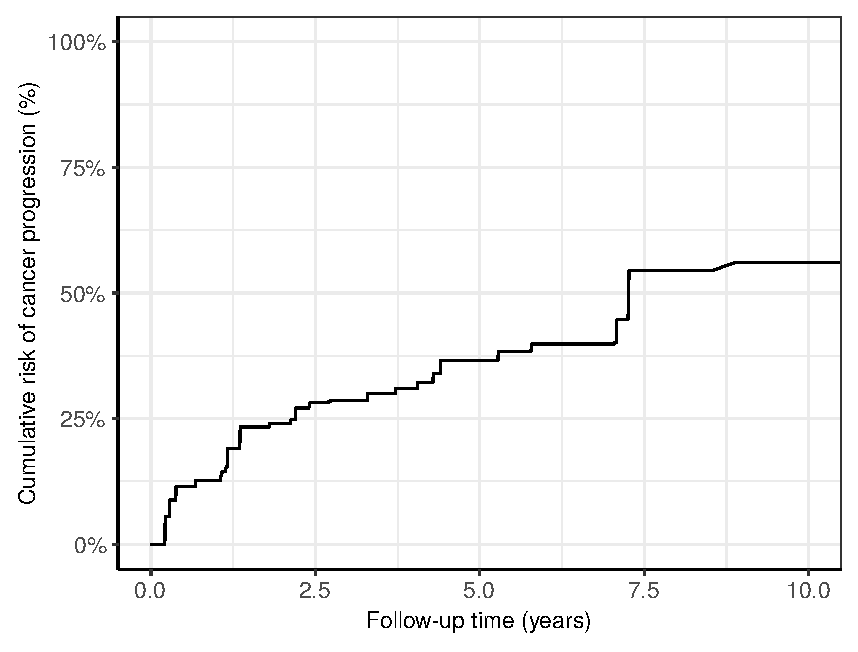
\includegraphics[width=\columnwidth]{images/npmle_plot.eps}}
\caption{\textbf{Estimated cumulative risk of cancer progression in AS} for patients in the Prostate Cancer Research International Active Surveillance (PRIAS) dataset. Nearly 50\% patients (\textit{slow progressing}) do not progress in the ten year follow-up period. Cumulative risk is estimated using nonparametric maximum likelihood estimation \citep{turnbull1976empirical}, to account for interval censored cancer progression times observed in the PRIAS dataset. Censoring includes death, removal from AS on the basis of observed longitudinal data, and patient dropout.}
\label{fig:npmle_plot}
\end{figure}

For all patients, PSA measurements (ng/mL) are scheduled every 3 months for the first 2 years and every 6 months thereafter. The DRE measurements are scheduled every 6 months. We use the DRE measurements as $\mbox{DRE} = \mbox{T1c}$ versus $\mbox{DRE} > \mbox{T1c}$. A DRE measurement equal to T1c\cite{schroder1992tnm} indicates a clinically inapparent tumor which is not palpable or visible by imaging, while tumors with $\mbox{DRE} > \mbox{T1c}$ are palpable.

\textbf{Data Accessibility:} The PRIAS database is not openly accessible. However, access to the database can be requested on the basis of a study proposal approved by the PRIAS steering committee. The website of the PRIAS program is \url{www.prias-project.org}.



\subsection{A Bivariate Joint Model for the Longitudinal PSA, and DRE Measurements, and Time of Cancer Progression}
Let $T_i^*$ denote the true cancer progression time of the ${i\mbox{-th}}$ patient included in PRIAS. Since biopsies are conducted periodically, $T_i^*$ is observed with interval censoring ${l_i < T_i^* \leq r_i}$. When progression is observed for the patient at his latest biopsy time $r_i$, then $l_i$ denotes the time of the second latest biopsy. Otherwise, $l_i$ denotes the time of the latest biopsy and ${r_i=\infty}$. Let $\boldsymbol{y}_{di}$ and $\boldsymbol{y}_{pi}$ denote his observed DRE and PSA longitudinal measurements, respectively. The observed data of all $n$ patients is denoted by ${\mathcal{D}_n = \{l_i, r_i, \boldsymbol{y}_{di}, \boldsymbol{y}_{pi}; i = 1, \ldots, n\}}$.

\begin{figure}[!htb]
\captionsetup{justification=justified}
\centerline{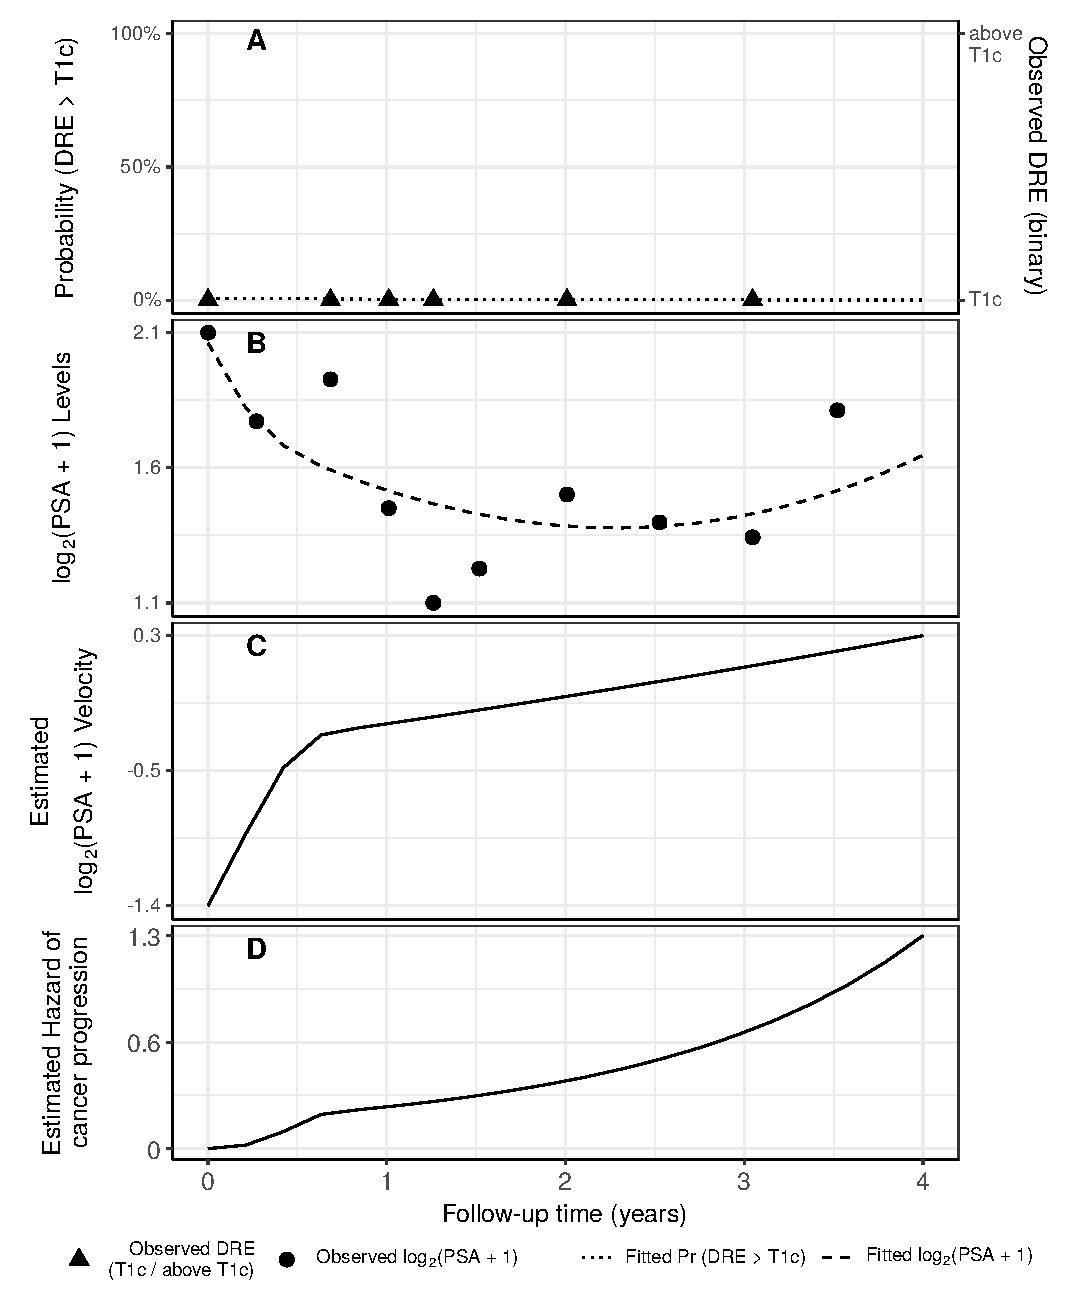
\includegraphics[width=\columnwidth]{images/jmExplanationPlot_1757.eps}}
\caption{\textbf{Illustration of the joint model fitted to the PRIAS dataset}. \textbf{Panel~A:} shows the observed DRE measurements and the fitted probability of obtaining $\mbox{DRE} > \mbox{T1c}$ (Equation~\ref{eq:long_model_dre}) for $i$-th patient. \textbf{Panel~B:} shows the observed and fitted $\log_2(\mbox{PSA} + 1)$ measurements (Equation~\ref{eq:long_model_psa}). \textbf{Panel~C:} shows the estimated $\log_2(\mbox{PSA} + 1)$ velocity (velocity cannot be observed directly) over time. The hazard function (Equation~\ref{eq:rel_risk_model}) shown in \textbf{Panel~D}, depends on the fitted log odds of having a $\mbox{DRE} > \mbox{T1c}$, and the fitted $\log_2(\mbox{PSA} + 1)$ value and velocity.}
\label{fig:jmExplanationPlot_1757}
\end{figure}

In our joint model, the patient-specific DRE and PSA measurements over time are modeled using a bivariate generalized linear mixed effects sub-model. The sub-model for DRE is given by (see~Panel~A, Figure~\ref{fig:jmExplanationPlot_1757}):
\begin{equation}
\label{eq:long_model_dre}
\begin{split}
    \mbox{logit} \big[\mbox{Pr}\{y_{di}(t) > \mbox{T1c}\}\big] &= \beta_{0d} + b_{0di} + (\beta_{1d} + b_{1di}) t\\
    &+ \beta_{2d} (\mbox{Age}_i-70) + \beta_{3d} (\mbox{Age}_i-70)^2
    \end{split}
\end{equation}
where, $t$ denotes the follow-up visit time, and $\mbox{Age}_i$ is the age of the ${i\mbox{-th}}$ patient at the time of inclusion in AS. We have centered the Age variable around the median age of 70 years for better convergence during parameter estimation. However, this does not change the interpretation of the parameters corresponding to the Age variable. The fixed effect parameters are denoted by ${\{\beta_{0d}, \ldots, \beta_{3d}\}}$, and ${\{b_{0di}, b_{1di}\}}$ are the patient specific random effects. With this definition, we assume that the patient-specific log odds of obtaining a DRE measurement larger than T1c remain linear over time. 

The mixed effects sub-model for PSA is given by (see~Panel~B, Figure~\ref{fig:jmExplanationPlot_1757}):
\begin{equation}
\label{eq:long_model_psa}
\begin{split}
    \log_2 \big\{y_{pi}(t) + 1\big\} &= m_{pi}(t) + \varepsilon_{pi}(t),\\
    m_{pi}(t) &= \beta_{0p} + b_{0pi} + \sum_{k=1}^4 (\beta_{kp} + b_{kpi})  B_k(t,\mathcal{K})\\ 
    &+ \beta_{5p} (\mbox{Age}_i-70) + \beta_{6p} (\mbox{Age}_i-70)^2,
    \end{split}
\end{equation}
where, $m_{pi}(t)$ denotes the underlying measurement error free value of $\log_2 (\mbox{PSA} + 1)$ transformed \citep{pearson1994mixed,lin2000latent} measurements at time $t$. We model it non-linearly over time using B-splines \citep{de1978practical}. To this end, our B-spline basis function $B_k(t, \mathcal{K})$ has 3 internal knots at $\mathcal{K} = \{0.1, 0.7, 4\}$ years, and boundary knots at 0 and 5.42 years (95-th percentile of the observed follow-up times). This specification allows fitting the $\log_2 (\mbox{PSA} + 1)$ levels in a piecewise manner for each patient separately. The internal and boundary knots specify the different time periods (analogously pieces) of this piecewise curve. The fixed effect parameters are denoted by ${\{\beta_{0p},\ldots,\beta_{6p}\}}$, and ${\{b_{0pi}, \ldots, b_{4pi}\}}$ are the patient specific random effects. The error $\varepsilon_{pi}(t)$ is assumed to be t-distributed with three degrees of freedom (see~Appendix~B.1) and scale $\sigma$, and is independent of the random effects. 

To account for the correlation between the DRE and PSA measurements of a patient, we link their corresponding random effects. More specifically, the complete vector of random effects ${\boldsymbol{b}_i = (b_{0di}, b_{1di}, b_{0pi}, \ldots, b_{4pi})^T}$ is assumed to follow a multivariate normal distribution with mean zero and variance-covariance matrix $\boldsymbol{D}$.

To model the impact of DRE and PSA measurements on the risk of cancer progression, our joint model uses a relative risk sub-model. More specifically, the hazard of cancer progression $h_i(t)$ at a time $t$ is given by (see~Panel~D, Figure~\ref{fig:jmExplanationPlot_1757}):
\begin{equation}
\label{eq:rel_risk_model}
\begin{split}
    h_i(t) &= h_0(t) \exp\Big(\gamma_1 (\mbox{Age}_i-70) + \gamma_2 (\mbox{Age}_i-70)^2\\
    &+\alpha_{1d} \mbox{logit} \big[\mbox{Pr}\{y_{di}(t) > \mbox{T1c}\}\big]+ \alpha_{1p} m_{pi}(t) + \alpha_{2p} \frac{\partial m_{pi}(t)}{\partial {t}}\Big),
    \end{split}
\end{equation}
where, $\gamma_1, \gamma_2$ are the parameters for the effect of age. The parameter $\alpha_{1d}$ models the impact of log odds of obtaining a $\mbox{DRE} > \mbox{T1c}$ on the hazard of cancer progression. The impact of PSA on the hazard of cancer progression is modeled in two ways: a) the impact of the error free underlying PSA value $m_{pi}(t)$ (see~Panel~B, Figure~\ref{fig:jmExplanationPlot_1757}), and b) the impact of the underlying PSA velocity $\partial m_{pi}(t)/\partial {t}$ (see~Panel~C, Figure~\ref{fig:jmExplanationPlot_1757}). The corresponding parameters are $\alpha_{1p}$ and $\alpha_{2p}$, respectively. Lastly, $h_0(t)$ is the baseline hazard at time $t$, and is modeled flexibly using P-splines \citep{eilers1996flexible}. The detailed specification of the baseline hazard $h_0(t)$, and the joint parameter estimation of the two sub-models using the Bayesian approach (R package \textbf{JMbayes}\cite{rizopoulosJMbayes}) are presented in Appendix A of the supplementary material.

% !TEX root =  ../main_manuscript.tex

\subsection{Personalized Decisions for Biopsy}
\label{subsec:pers_decision_making}
Let us assume that a decision of conducting a biopsy is to be made for a new patient $j$ shown in Figure~\ref{fig:obsDataPlot_2340}, at his current follow-up visit time $s$. Let $t\leq s$ be the time of his latest negative biopsy. Let $\mathcal{Y}_{dj}(s)$ and $\mathcal{Y}_{pj}(s)$ denote his observed DRE and PSA measurements up to the current visit, respectively. From the observed measurements we want to extract the underlying measurement error free trend of $\log_2 (\mbox{PSA} + 1)$ values and velocity, and the log odds of obtaining $\mbox{DRE} > \mbox{T1c}$. We intend to combine them to inform us when the cancer progression is to be expected (see Figure~\ref{fig:dynRiskPlot_2340}), and to further guide the decision making on whether to conduct a biopsy at the current follow-up visit. The combined information is given by the following posterior predictive distribution $g(T^*_j)$ of his time of cancer progression $T^*_j > t$ (see Appendix~A.4 for details):
\begin{equation}
\label{eq:post_pred_dist}
g(T^*_j) = p\big\{T^*_j \mid T^*_j > t, \mathcal{Y}_{dj}(s), \mathcal{Y}_{pj}(s), \mathcal{D}_n\big\}.
\end{equation}
The distribution $g(T^*_j)$ is not only patient-specific, but also updates as extra information is recorded at future follow-up visits.

\begin{figure}[!htb]
\captionsetup{justification=justified}
\centerline{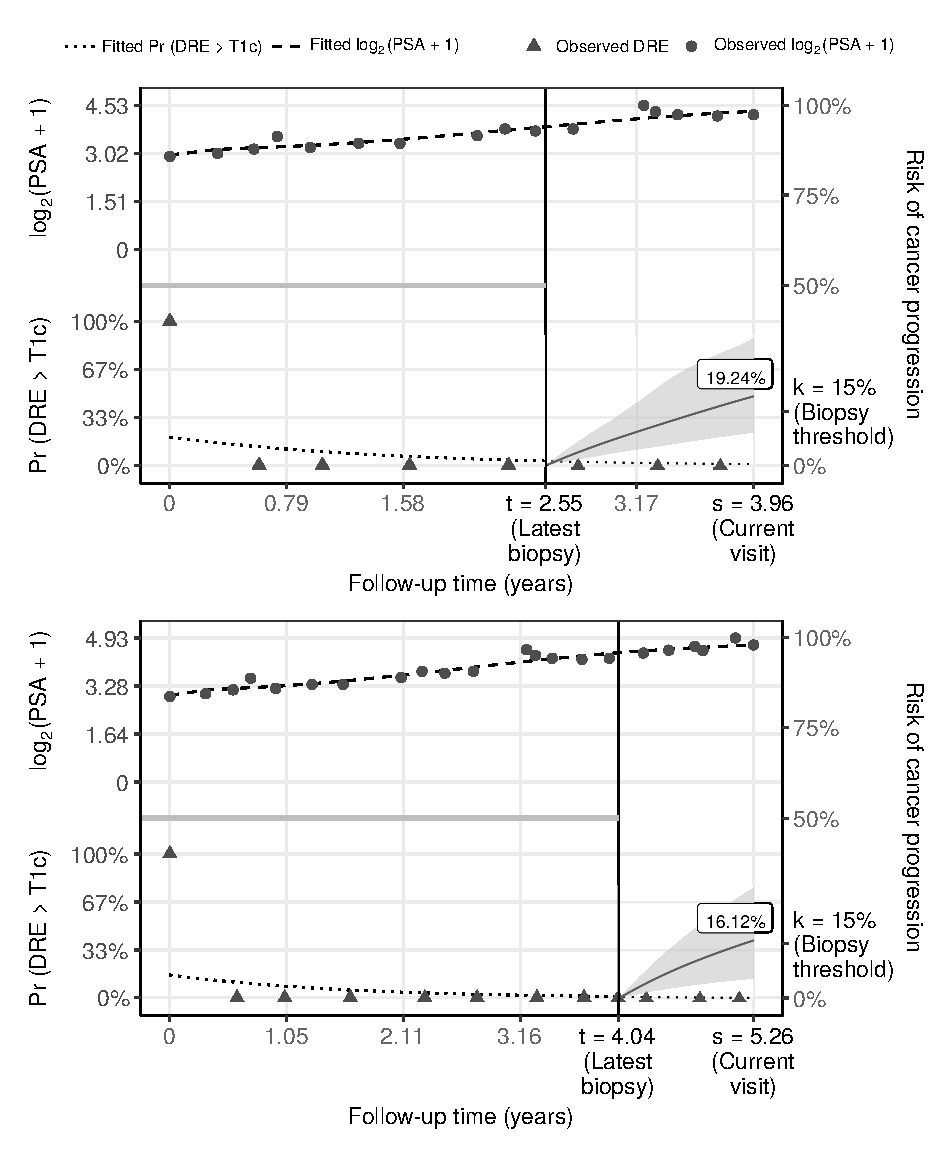
\includegraphics[width=\columnwidth]{images/dynRiskPlot_2340.eps}}
\caption{\textbf{Illustration of personalized decision of biopsy} for patient $j$ at two different follow-up visits. Biopsy is recommended if the personalized cumulative risk of cancer progression estimated from the joint model fitted to the observed data of the patient, is higher than the example risk threshold for biopsy ($\kappa=$ 10\%). \textbf{Panel~A:} biopsy is not recommended for the patient $j$ at the follow-up visit time $s=4$ years, because his estimated personalized cumulative risk of cancer progression (7.8\%) is less than the threshold. \textbf{Panel~B:} biopsy is recommended for the patient $j$ at the follow-up visit time $s=5.3$ years, because his estimated personalized cumulative risk of cancer progression (13.5\%) is more than the threshold.}
\label{fig:dynRiskPlot_2340}
\end{figure}

A key ingredient in the decision of conducting a biopsy for patient $j$ at the current follow-up visit time $s$ is the personalized cumulative risk of observing a cancer progression at time $s$ (illustrated in Figure~\ref{fig:dynRiskPlot_2340}). This risk can be derived from the posterior predictive distribution $g(T^*_j)$ \cite{rizopoulos2011dynamic}, and is given by:
\begin{equation}
\label{eq:dynamic_risk_prob}
R_j(s \mid t) = \mbox{Pr}\big\{T^*_j \leq s \mid T^*_j > t, \mathcal{Y}_{dj}(s), \mathcal{Y}_{pj}(s), \mathcal{D}_n\big\}, \quad s \geq t.
\end{equation}
A simple and straightforward approach to decide upon conducting a biopsy for patient $j$ at the current follow-up visit would be to do so if his personalized cumulative risk of cancer progression at the visit is higher than a certain threshold $0 \leq \kappa \leq 1$. For example, as shown in Panel~B of Figure~\ref{fig:dynRiskPlot_2340}, biopsy at a visit may be scheduled if the personalized cumulative risk is higher than 10\% (example risk threshold). This decision making process is iterated over the follow-up period, incorporating on each subsequent visit the newly observed data, until a positive biopsy is observed. Subsequently, an entire personalized schedule of biopsies for each patient can be obtained.

%Although, the number of unnecessary biopsies a risk threshold may eventually lead to is related to its accuracy of classification between patients whose cancers have progressed and patients without cancer progression. The classification accuracy of a risk threshold also varies over the follow-up period.

The choice of the risk threshold dictates the schedule of biopsies and has to be made on each subsequent follow-up visit of a patient. In this regard, a straightforward approach is choosing a fixed risk threshold, such as 5\% or 10\% risk, at all follow-up visits. Fixed risk thresholds may be chosen by patients and/or doctors according to how they weigh the relative harms of doing an unnecessary biopsy versus a missed cancer progression (e.g., 10\% threshold means a 1:9 ratio) if the biopsy is not conducted \cite{vickers2006decision}. An alternative approach is that at each follow-up visit a unique threshold is chosen on the basis of its classification accuracy. More specifically, given the time of latest biopsy $t$ of patient $j$, and his current visit time $s$\, we find a visit-specific biopsy threshold $\kappa$, which gives the highest cancer progression detection rate (true positive rate, or TPR) for the period $(t, s]$. However, we also intend to balance for unnecessary biopsies (high false positive rate), or a low number of correct detections (high false negative rate) when the false positive rate is minimized. An approach to mitigate these issues is to maximize the TPR and positive predictive value (PPV) simultaneously. To this end, we utilize the $\mbox{F}_1$ score, which is a composite of both TPR and PPV (estimated as in Rizopoulos~et~al., 2017 \cite{landmarking2017}), and is defined as: 
\begin{equation}
\label{eq:F1_TPR_PPV}
\begin{split}
\mbox{F}_1(t,  s, \kappa) &= 2\frac{\mbox{TPR}(t,  s, \kappa)\ \mbox{PPV}(t,  s, \kappa)}{\mbox{TPR}(t,  s, \kappa) + \mbox{PPV}(t,  s, \kappa)},\\
\mbox{TPR}(t,  s, \kappa) &= \mbox{Pr}\big\{R_j(s \mid t) > \kappa \mid t < T^*_j \leq s\big\},\\
\mbox{PPV}(t,  s, \kappa) &= \mbox{Pr}\big\{t < T^*_j \leq s \mid R_j(s \mid t) > \kappa \big\}.
\end{split}
\end{equation}
The $\mbox{F}_1$ score ranges between 0 and 1, where a value of 1 signifies perfect TPR and PPV. Since a high $\mbox{F}_1$ score is desired, the visit-specific threshold ${\kappa=\argmax_{\kappa} \mbox{F}_1(t, s, \kappa)}$. The criteria on which we evaluate the personalized schedules based on fixed risk threshold at all visits, as well as visit-specific risk threshold using $\mbox{F}_1$ score, is the total number of biopsies scheduled, and the delay in detection of cancer progression (details in \hyperref[sec:results]{Results}). 
% !TEX root =  ../main_manuscript.tex

\subsection{Simulation Study}
\label{subsec:sim_study}
Although the personalized decision making approach is motivated by the PRIAS study, it is not possible to evaluate it on the PRIAS dataset. This is because the patients in PRIAS have already had their biopsies as per the PRIAS protocol. In addition, the true time of cancer progression is interval or right censored for all patients, making it impossible to correctly estimate the delay in detection of cancer progression due to a particular schedule. To this end, we conduct an extensive simulation study to find the utility of personalized, PRIAS, and fixed/heuristic schedules. For a realistic comparison, we simulate data from the joint model fitted to the PRIAS dataset. The simulated population has the same ten year follow-up period as the PRIAS study. In addition, the estimated relations between DRE and PSA measurements, and the risk of cancer progression are retained in the simulated population.

From this population, we first sample 500 datasets, each representing a hypothetical AS program with 1000 patients in it. We generate a true cancer progression time for each of the ${\mbox{500} \times \mbox{1000}}$ patients, and then sample a set of DRE and PSA measurements at the same follow-up visit times as given in PRIAS protocol. We then split each dataset into a training (750 patients) and a test (250 patients) part, and generate a random and non‐informative censoring time for the training patients. We next fit a joint model of the specification given in Equations (\ref{eq:long_model_dre}), (\ref{eq:long_model_psa}), and (\ref{eq:rel_risk_model}) to each of the 500 training datasets and obtain MCMC samples from the 500 sets of the posterior distribution of the parameters. 

In each of the 500 hypothetical AS programs, we utilize the corresponding fitted joint models to develop cancer progression risk profiles for each of the ${\mbox{500} \times \mbox{250}}$ test patients. We make the decision of biopsies for patients at their pre-scheduled follow-up visits for DRE and PSA measurements (see \hyperref[subsec:study_population]{Study Population}), on the basis of their visit and patient-specific estimated cumulative risk of cancer progression. These decisions are made iteratively until a positive biopsy is observed. A recommended gap of one year between consecutive biopsies\cite{bokhorst2015compliance} is also maintained. Subsequently, for each patient, an entire personalized schedule of biopsies is obtained.

We evaluate and compare both personalized and currently practiced schedules of biopsies in this simulation study. Comparison of the schedules is based on the number of biopsies scheduled and the corresponding delay in detection of cancer progression. We evaluate the following currently practiced fixed/heuristic schedules: biopsy annually, biopsy every one and a half years, biopsy every two years and biopsy every three years. We also evaluate the biopsy schedule of the PRIAS program (see \hyperref[sec:introduction]{Introduction}). For the personalized biopsy schedules, we evaluate schedules based on three fixed risk thresholds: 5\%, 10\% and 15\%, corresponding to a missed cancer progression being 19, 9, and 5.5 times more harmful than an unnecessary biopsy \cite{vickers2006decision}, respectively. We also implement a personalized schedule where a follow-up visit-specific risk threshold is chosen using $\mbox{F}_1$ score.

% !TEX root =  ../main_manuscript.tex 
\section{Demonstration of Personalized Schedules}
\label{sec:results}

% !TEX root =  ../main_manuscript.tex 
\section{Discussion}
\label{sec:discussion}
In this paper, we presented a methodology to create personalized schedules for burdensome diagnostic \textit{tests} utilized to detect disease \textit{progression} in early-stage chronic non-communicable disease \textit{surveillance}. For this purpose, we utilized joint models for time-to-event and longitudinal data. Our approach first combines a patient's clinical data (e.g., longitudinal biomarkers) and previous invasive test results to estimate patient-specific cumulative-risk of disease progression over their current and future follow-up visits. We then plan future invasive tests whenever this cumulative-risk of progression is predicted to be above a certain threshold. We select the risk threshold automatically in a personalized manner, by optimizing a utility function of the patient-specific consequences of choosing a particular risk threshold based schedule. These consequences are, namely, the number of invasive tests (burden) planned in a schedule, and the expected time delay in detection of progression (shorter is beneficial) if the patient progresses. Last, we calculate this expected time delay in a personalized manner for both personalized and fixed schedules to assist patients/doctors in making a more informed decision of choosing a test schedule.

Using joint models gives us certain advantages. First, since joint models employ random-effects, the corresponding risk-based schedules are inherently personalized. Second, to predict this patient-specific risk of progression, joint models utilize all observed longitudinal measurements of a patient. Also, the continuous longitudinal outcomes are not discretized, which is commonly a case in Markov Decision Process and flowchart-based test schedules. Third, personalized schedules update automatically with more patient data over follow-up. Fourth, we calculated the expected number of tests (burden) and expected time delay in detecting progression (shorter is beneficial) in a patient-specific manner. Using our methodology, these can be calculated for both personalized and fixed schedules. Thus, patients/doctors can compare risk-based and fixed schedules and choose one according to their preferences for the expected burden-benefit ratio. Last, although this work concerns invasive test schedules in disease surveillance, the methodology is generic for use under a screening setting as well.

Personalized schedules that we proposed require a risk threshold. We optimized the threshold choice using a generic utility function based on the expected number of biopsies and time delay in detecting progression. We used only these two measures because they are easy to interpret but simultaneously critical for deciding the timing of invasive tests. Also, the time delay in detecting progression should manifest the window of opportunity for curative treatment and additional benefits of observing progression early. Practitioners may extend/modify this utility function by adding to/replacing time delay with commonly used decision-theoretic measures such as quality-adjusted life-years/expectancy (QALY/QALE).

We evaluated personalized schedules in a full cohort via a realistic simulation of a randomized clinical trial for prostate cancer surveillance patients. We observed that personalized schedules reduced many unnecessary biopsies for non-progressing patients compared to the widely used annual schedule. This happened at the cost of simultaneously having a slightly more time delay in detecting progression. Although, this delay should still be safe because it was almost equal to the delay of the world's largest prostate cancer active surveillance program PRIAS's schedule. The simulation study results are by no means the performance-limit of the personalized schedules. Instead, models with higher predictive accuracy and discrimination capacity than the PRIAS based model may lead to an even better balance between the number of tests and the time delay in detecting progression.

There are certain limitations to this work. First, in practice, most cohorts have a limited study period. Hence, the cumulative-risk profiles of patients and resulting personalized schedules can only be created up to the maximum study period. For this problem, the risk prediction model should be updated with more follow-up data over time. The proposed joint model assumed all events other than progression to be non-informative censoring. Alternative models that account for competing risks may lead to better results as they estimate absolute and not the cause-specific risk of progression. Upgrading is susceptible to inter-observer variation and sampling error. Although models that account for these two issues~\citep{balasubramanian2003estimation,coley2017prediction} will provide better risk estimates, the methodology for obtained personalized schedules can remain the same.

% !TEX root =  main_manuscript.tex

\section*{Acknowledgements}
The first and last authors would like to acknowledge support by the Netherlands Organization for Scientific Research's VIDI grant nr. 016.146.301, and Erasmus MC funding. The authors also thank the Erasmus MC Cancer Computational Biology Center for giving access to their IT-infrastructure and software that was used for the computations and data analysis in this study. Lastly, we thank Frank-Jan H. Drost from the Department of Urology, Erasmus University Medical Center, for helping us in accessing the PRIAS data set. \vspace*{-8pt}

\begin{sm}
Supplementary material for this article, containing Appendix A--D are available in the file `supplementary.pdf'.
\end{sm} 

\bibliographystyle{SageV}
\bibliography{bibliography.bib}

\end{document}


